\section{Die Simulation}
\begin{figure}
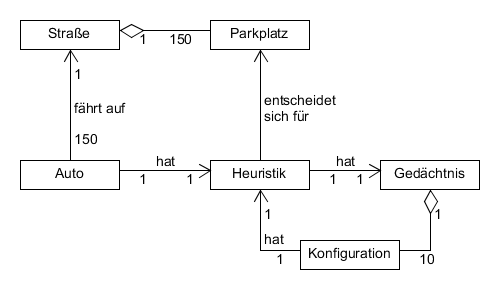
\includegraphics[width=0.5\textwidth]{uml/simOverview.png}
\caption{Strukturelle Übersicht der Simulation}\label{fig_simOver}
\end{figure}
Um die Konfigurationen für die Heuristiken zu lernen wird die Parkplatzsuche simuliert. Da in dieser Arbeit mehrere Fragen beantwortet werden sollen, sind auch mehrere Simulationen mit unterschiedlichen Randbedingungen notwendig. Der Grundlegende Aufbau jeder Simulation ist jedoch gleich und in Abbildung \ref{fig_simOver} dargestellt. Die Simulation ist objekt-orientiert aufgebaut. Die Straße verwaltet dabei sowohl die Autos und die Parkplätze als auch die diskreten zeitschritte der Simulation. Autos fahren zu einem zufälligen Zeitpunkt in die Straße ein und erreichen in jedem Zeitschritt, im Folgenden \emph{tick} genannt, einen Parkplatz. Dieser wird von der Heuristik des Autos, die man als den Fahrer des Autos interpretieren kann, evaluiert diesen Parkplatz, sofern er noch nicht belegt ist. Entscheidet sich die Heuristik für den Parkplatz parkt auch das Auto für eine bestimmte Zeit auf ihm. Das Ausparken wird nur durch die Freigabe des Parkplatzes nach der Parkzeit des Autos modelliert. Um zu garantieren, dass immer Parkplätze gefunden werden, werden in den Simulationen genausoviele Autos eingesetzt wie Parkplätze vorhanden sind. Die genaue Implementierung wird im Anhang erläutert.

\subsection{Wahl der Parameter}
Jede der durchgeführten Simulationen hat eine Dauer von $10^7$ Ticks und eine Straße mit $150$ Parkplätzen. Die Topologie der Straße, siehe Abbildung \ref{fig_street}, ist von Hutchinson et al \textbf{cite} übernommen. Die Straße verläuft \emph{U-förmig} mit einem gemeinsamen Ziel für alle Autos im Scheitelpunkt und einer beidseitig zugänglichen Parkfläche in der Mitte. Die Topologie ähnelt also einem Supermarktparkplatz. 
\begin{figure}
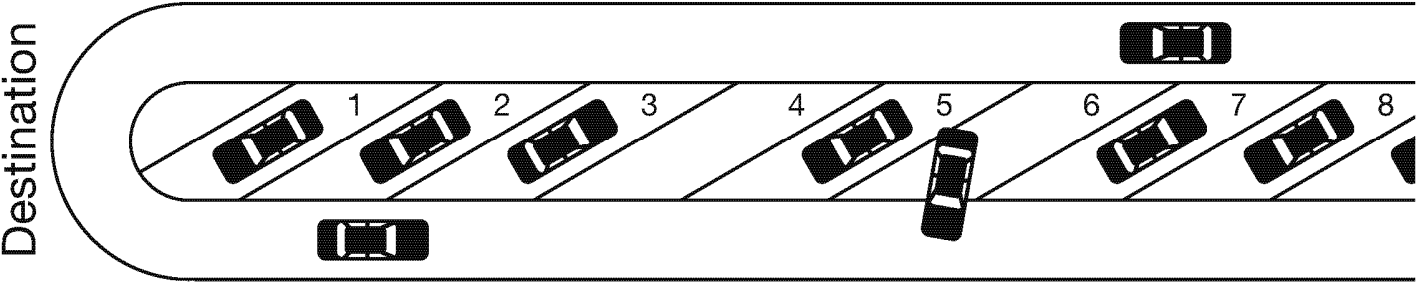
\includegraphics[width=\textwidth]{pics/street.png}
\caption{textbf{cite}, Topologie der Straße}\label{fig_street}
\end{figure}
 Die Parkfläche hat eine Länge von $150$ Parkplätzen. Weiterhin wird die Dauer der diskreten Zeitschritte über die Parkplätze definiert. Ein \emph{Tick} ist die Zeit, die ein Auto benötigt, um einen Parkplatz zu passieren. 
In Anlehnung an Hutchinson et al beträgt deren Breite $5m$. Jedoch sind die dort angegeben $22,5 km/h$ zu schnell um gefahrlos auf Parkplätzen gefahren zu werden. Stattdessen wird in der hier beschriebenen Simulation eine Geschwindkeit von $12km/h$ angenommen. Dies erhöht die Dauer eines \emph{Ticks} von $0.75s$ auf $1,5s$. Die Fahrbahn besitzt demnach eine Länge von $301$ \emph{Ticks}, einem mehr als in der Vorlage. Das Durchqueren des Scheitelpunktes ist auch in der Realtät nicht instantan, was den zusätzlichen \emph{Tick} im Scheitelpunkt bedingt. 

Die Wartezeit zwischen zwei Autos ist in der Simulation gleichverteilt. Die untere Schranke ist dabei immer $0$. Über die obere Schranke wird die Verkehrsdichte modelliert. Ein niedrigerer Wert resultiert dabei in einem höheren Verkehrsaufkommen. Da sich die Verkehrsdichten im Laufe eines Tages ändern wurden für die Zeiten \emph{Morgen}, \emph{Mittag} und \emph{Abend} die oberen Wartezeitschranken $40$, $80$ und $20$ \emph{Ticks} festgelegt. Dies entspricht jeweils $2$, einem und $4$ Autos pro Minute. Interpretativ hat man so die Morgeneinkäufe, die Mittagsflaute und den Feierabendverkehr. 

Wählt ein Auto einen Parkplatz aus, parkt es auf diesem. Der Parkplatz kann für eine bestimmte Zeit nicht von anderen Autos ausgewähöt werden. Die Parkdauer in dieser Simulation auf einer Normalverteilung mit Mittelwert $E=1h$ und Standardabweichung $\sigma = 0,5h$. Die Gesamtparkdauer wird durch 
\begin{align}
t_{gesamt} &= 2\cdot 2\cdot d + N(X)
\end{align}
bestimmt. Dabei ist $d$ die Entfernung des Parkplatzes zum Ziel. Es wird analog zu Hutchinson et al angenommen, dass Fußgänger sich mit halber Geschwindigkeit fortbewegen. Die Strecke zwischen Parkplatz und Ziel muss zudem sowohl auf dem Hinweg als auch auf dem Rückweg absolviert werden.

Es werden die folgenden Simulationen ausgewertet:
\begin{enumerate}
	\item Für jede Heuristik und jede Verkehrsdichte eine Simulation, in der es genau ein Auto mit der jeweiligen Heuristik gibt. Die restliche Population wählt einen Parkplatz zufällig. Dabei ist es wahrscheinlicher einen Parkplatz zu nehmen desto näher dieser am Ziel ist.
	\item Eine Simulation, bei der $20\%$ der Population eine der betrachteten Heuristiken erhalten. Jede Heuristik wird dann in insgesamt $5$ Autos verwendet. Der Rest der Population wählt einen Parkplatz wieder wie oben zufällig. 
	\item Eine Simulation, bei der jedes Auto eine Strategie verfolgt. Der Anteil der Autos mit einer Heuristik beträgt also $100\%$.
\end{enumerate}
Damit die Heuristiken genügend Zeit zum Lernen haben dauert jede der Simulationen $10^7$ \emph{Ticks}. Dies führt, je nach zugrunde liegender Verkehrsdichte, zu etwa $1500$ bis $4500$ Lernschritten. 
